%%%%%%%%%%%%%%%%%%%%%%%%%%%%%%%%%%%%%%%%%
% Large Colored Title Article
% LaTeX Template
% Version 1.1 (25/11/12)
%
% This template has been downloaded from:
% http://www.LaTeXTemplates.com
%
% Original author:
% Frits Wenneker (http://www.howtotex.com)
%
% License:
% CC BY-NC-SA 3.0 (http://creativecommons.org/licenses/by-nc-sa/3.0/)
%
%%%%%%%%%%%%%%%%%%%%%%%%%%%%%%%%%%%%%%%%%

%----------------------------------------------------------------------------------------
%	PACKAGES AND OTHER DOCUMENT CONFIGURATIONS
%----------------------------------------------------------------------------------------

\documentclass[DIV=calc, paper=a4, fontsize=11pt, twocolumn]{scrartcl}	 % A4 paper and 11pt font size
\usepackage{etex}
\usepackage{lipsum} % Used for inserting dummy 'Lorem ipsum' text into the template
\usepackage[english]{babel} % English language/hyphenation
\usepackage[protrusion=true,expansion=true]{microtype} % Better typography
\usepackage{amsmath,amsfonts,amsthm} % Math packages
\usepackage[svgnames]{xcolor} % Enabling colors by their 'svgnames'
\usepackage[hang, small,labelfont=bf,up,textfont=it,up]{caption} % Custom captions under/above floats in tables or figures
\usepackage{booktabs} % Horizontal rules in tables
\usepackage{fix-cm}	 % Custom font sizes - used for the initial letter in the document

\usepackage{algorithmic}
\usepackage{algorithm}
\usepackage{html}
\usepackage{slashbox} % table cell diagonal split
\usepackage{url}
\usepackage{graphicx}
\usepackage{wrapfig}
\usepackage{array}
\usepackage{longtable}
\usepackage{color}
\usepackage{microtype}    % improves, among other things, line-breaks in narrow columns
\usepackage{enumitem}
\usepackage{eucal}
\usepackage{tikz-qtree} 	% drawing hierarchies

\usepackage[disable]{todonotes} % To remove in-line review comments, use 'disable'
%\usepackage[colorinlistoftodos,textsize=normalsize,textwidth=1\marginparwidth]{todonotes} % To add in-line review comments

\usepackage{sectsty} % Enables custom section titles
\allsectionsfont{\usefont{OT1}{phv}{b}{n}} % Change the font of all section commands

\usepackage{fancyhdr} % Needed to define custom headers/footers
\pagestyle{fancy} % Enables the custom headers/footers
\usepackage{lastpage} % Used to determine the number of pages in the document (for "Page X of Total")

%\usepackage[disable]{todonotes} % To remove in-line review comments, use 'disable'
%\usepackage[colorinlistoftodos,textsize=normalsize,textwidth=1\marginparwidth]{todonotes} % To add in-line review comments

% Headers - all currently empty
\lhead{}
\chead{}
\rhead{}

% Footers
\lfoot{}
\cfoot{}
\rfoot{\footnotesize Page \thepage\ of \pageref{LastPage}} % "Page 1 of 2"

\renewcommand{\headrulewidth}{0.0pt} % No header rule
\renewcommand{\footrulewidth}{0.4pt} % Thin footer rule

\usepackage{lettrine} % Package to accentuate the first letter of the text
\newcommand{\initial}[1]{ % Defines the command and style for the first letter
\lettrine[lines=3,lhang=0.3,nindent=0em]{
\color{DarkGoldenrod}
{\textsf{#1}}}{}}

%%----------------------------------------------------------------------------------------
%%	TITLE SECTION
%%----------------------------------------------------------------------------------------
%
%\usepackage{titling} % Allows custom title configuration
%
%\newcommand{\HorRule}{\color{DarkGoldenrod} \rule{\linewidth}{1pt}} % Defines the gold horizontal rule around the title
%
%\pretitle{\vspace{-30pt} \begin{flushleft} \HorRule \fontsize{50}{50} \usefont{OT1}{phv}{b}{n} \color{DarkRed} \selectfont} % Horizontal rule before the title
%
%\title{Article Title} % Your article title
%
%\posttitle{\par\end{flushleft}\vskip 0.5em} % Whitespace under the title
%
%\preauthor{\begin{flushleft}\large \lineskip 0.5em \usefont{OT1}{phv}{b}{sl} \color{DarkRed}} % Author font configuration
%
%\author{John Smith, } % Your name
%
%\postauthor{\footnotesize \usefont{OT1}{phv}{m}{sl} \color{Black} % Configuration for the institution name
%University of California % Your institution
%
%\par\end{flushleft}\HorRule} % Horizontal rule after the title
%
%\date{} % Add a date here if you would like one to appear underneath the title block
%
%%----------------------------------------------------------------------------------------
 % One pager
%%%%%%%%%%%%%%%%%%%%%%%%%%%%%%%%%%%%%%%%%%
% Large Colored Title Article
% LaTeX Template
% Version 1.1 (25/11/12)
%
% This template has been downloaded from:
% http://www.LaTeXTemplates.com
%
% Original author:
% Frits Wenneker (http://www.howtotex.com)
%
% License:
% CC BY-NC-SA 3.0 (http://creativecommons.org/licenses/by-nc-sa/3.0/)
%
%%%%%%%%%%%%%%%%%%%%%%%%%%%%%%%%%%%%%%%%%

%----------------------------------------------------------------------------------------
%	PACKAGES AND OTHER DOCUMENT CONFIGURATIONS
%----------------------------------------------------------------------------------------

%\documentclass[DIV=calc, paper=a4, fontsize=11pt, twocolumn]{scrartcl}	 % A4 paper and 11pt font size
\documentclass[DIV=calc, paper=a4, fontsize=11pt, twocolumn]{scrreprt}
\usepackage[english]{babel} % English language/hyphenation
%\usepackage[protrusion=true,expansion=true]{microtype} % XeTex Problem
\usepackage{amsmath,amsfonts,amsthm} % Math packages
\usepackage[svgnames]{xcolor} % Enabling colors by their 'svgnames'
\usepackage[hang, small,labelfont=bf,up,textfont=it,up]{caption} % Custom captions under/above floats in tables or figures
\usepackage{booktabs} % Horizontal rules in tables
\usepackage{fix-cm}	 % Custom font sizes - used for the initial letter in the document
\usepackage{epigraph}
\setlength{\epigraphwidth}{0.8\linewidth}
\setlength{\epigraphrule}{0pt}
\renewcommand*{\textflush}{flushright}
\renewcommand*{\epigraphsize}{\normalsize\itshape}


\usepackage{algorithmic}
\usepackage{algorithm}
\usepackage{html}
\usepackage{slashbox} % table cell diagonal split
\usepackage{url}
\usepackage{graphicx}
\usepackage{wrapfig}
\usepackage{array}
\usepackage{longtable}
\usepackage{color}
\usepackage{enumitem}
\usepackage{eucal}
\usepackage{tikz-qtree} 	% drawing hierarchies


\usepackage[disable]{todonotes} % To remove in-line review comments, use 'disable'
%\usepackage[colorinlistoftodos,textsize=normalsize,textwidth=1\marginparwidth]{todonotes} % To add in-line review comments

\usepackage{sectsty} % Enables custom section titles
%\allsectionsfont{\usefont{OT1}{phv}{b}{n}} % Change the font of all section commands

\usepackage{fancyhdr} % Needed to define custom headers/footers
\pagestyle{fancy} % Enables the custom headers/footers
\usepackage{lastpage} % Used to determine the number of pages in the document (for "Page X of Total")


\lhead{}
\chead{}
\rhead{}


\lfoot{}
\cfoot{}
\rfoot{\footnotesize Page \thepage\ of \pageref{LastPage}} % "Page 1 of 2"

\renewcommand{\headrulewidth}{0.0pt} % No header rule
\renewcommand{\footrulewidth}{0.4pt} % Thin footer rule

\usepackage{lettrine} % Package to accentuate the first letter of the text
\newcommand{\initial}[1]{ % Defines the command and style for the first letter
\lettrine[lines=3,lhang=0.3,nindent=0em]{
\color{DarkGoldenrod}
{\textsf{#1}}}{}}

\usepackage{titling} % Allows custom title configuration
\usepackage{subfig}
\usepackage[export]{adjustbox}
\usepackage{bbding}

\newcommand{\HorRule}{\color{DarkGoldenrod} \rule{\linewidth}{1pt}} % Defines the gold horizontal rule around the title
\pretitle{\vspace{-70pt} \begin{flushleft} \HorRule \fontsize{20}{20} \usefont{OT1}{phv}{b}{n} \color{DarkRed} \selectfont} % Horizontal rule before the title

\title{Computing Midsurface} % Your article title

\posttitle{\par\end{flushleft}\vskip 0.125em} % Whitespace under the title
\preauthor{
\begin{flushleft}\large \lineskip 0.5em \usefont{OT1}{phv}{b}{sl} \color{DarkRed}} % Author font configuration
\author{Yogesh Kulkarni\\} % Your name
\postauthor{\footnotesize \usefont{OT1}{phv}{m}{sl} \color{Black} % Configuration for the institution name
PhD, College of Engineering Pune, India. % Your institution
\quad \Envelope \ yogeshkulkarni@yahoo.com \quad \Phone \ +91 9890251406
\vspace{-4mm}
\end{flushleft}\HorRule} % Horizontal rule after the title

\date{} % Add a date here if you would like one to appear underneath the title block

%----------------------------------------------------------------------------------------

\begin{document}

\maketitle

\vspace{-8mm}
\section{Introduction}
Thin-walled Computer-aided Design (CAD) models of sheet metal/plastic parts are often simplified and reduced dimensionally to \textbf{Midsurface} (a surface running through the part, midway of the thickness) before analyzing them in Computer-aided Engineering (CAE), to save on compute time and resources. 
\begin{center}
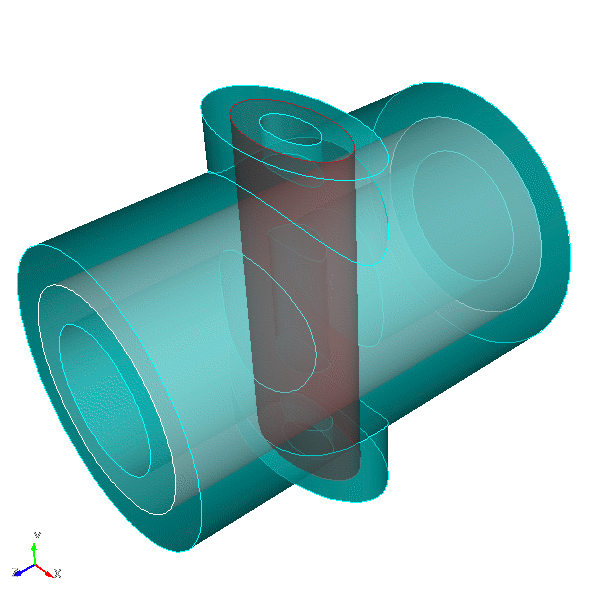
\includegraphics[width=0.7\linewidth]{../Common/images/MidsurfaceTitle}
\end{center}

Extraction of the midsurface is still, mostly, a manual and time-consuming process due to lack of robust and automated methods, especially for the complex models. Existing methods result in failures such as gaps, overlaps, voids, etc., which take hours or even days to correct manually. 

\begin{center}
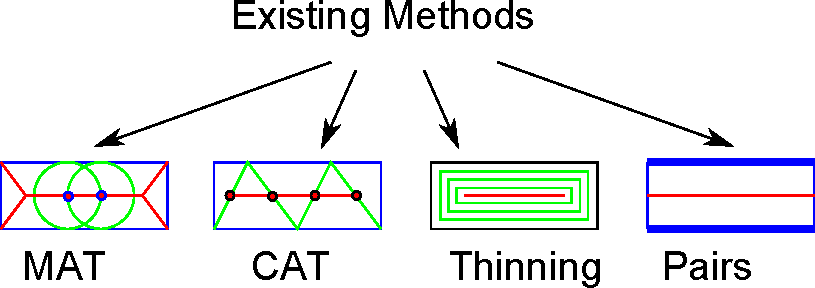
\includegraphics[width=0.9\linewidth]{../Common/images/MedialMethodsOnly.pdf}
\end{center}

Methods shown above have quite a few problems. MAT suffers from extraneous branches and ``Pairs'' suffers from complexity in finding the face pairs. CAT and Thinning leave gaps at ends. 
Fundamental reason for these problems is that these methods work on the final shape, in which it is challenging to decipher interactions amongst the sub-shapes needed for the computation of well-connected midsurface.


\section{Proposed Approach}

 Decomposing the final shape into smaller-simpler shapes, in form of cellular features, makes computation of midsurface more deterministic. 
 
\vspace{0.5em}

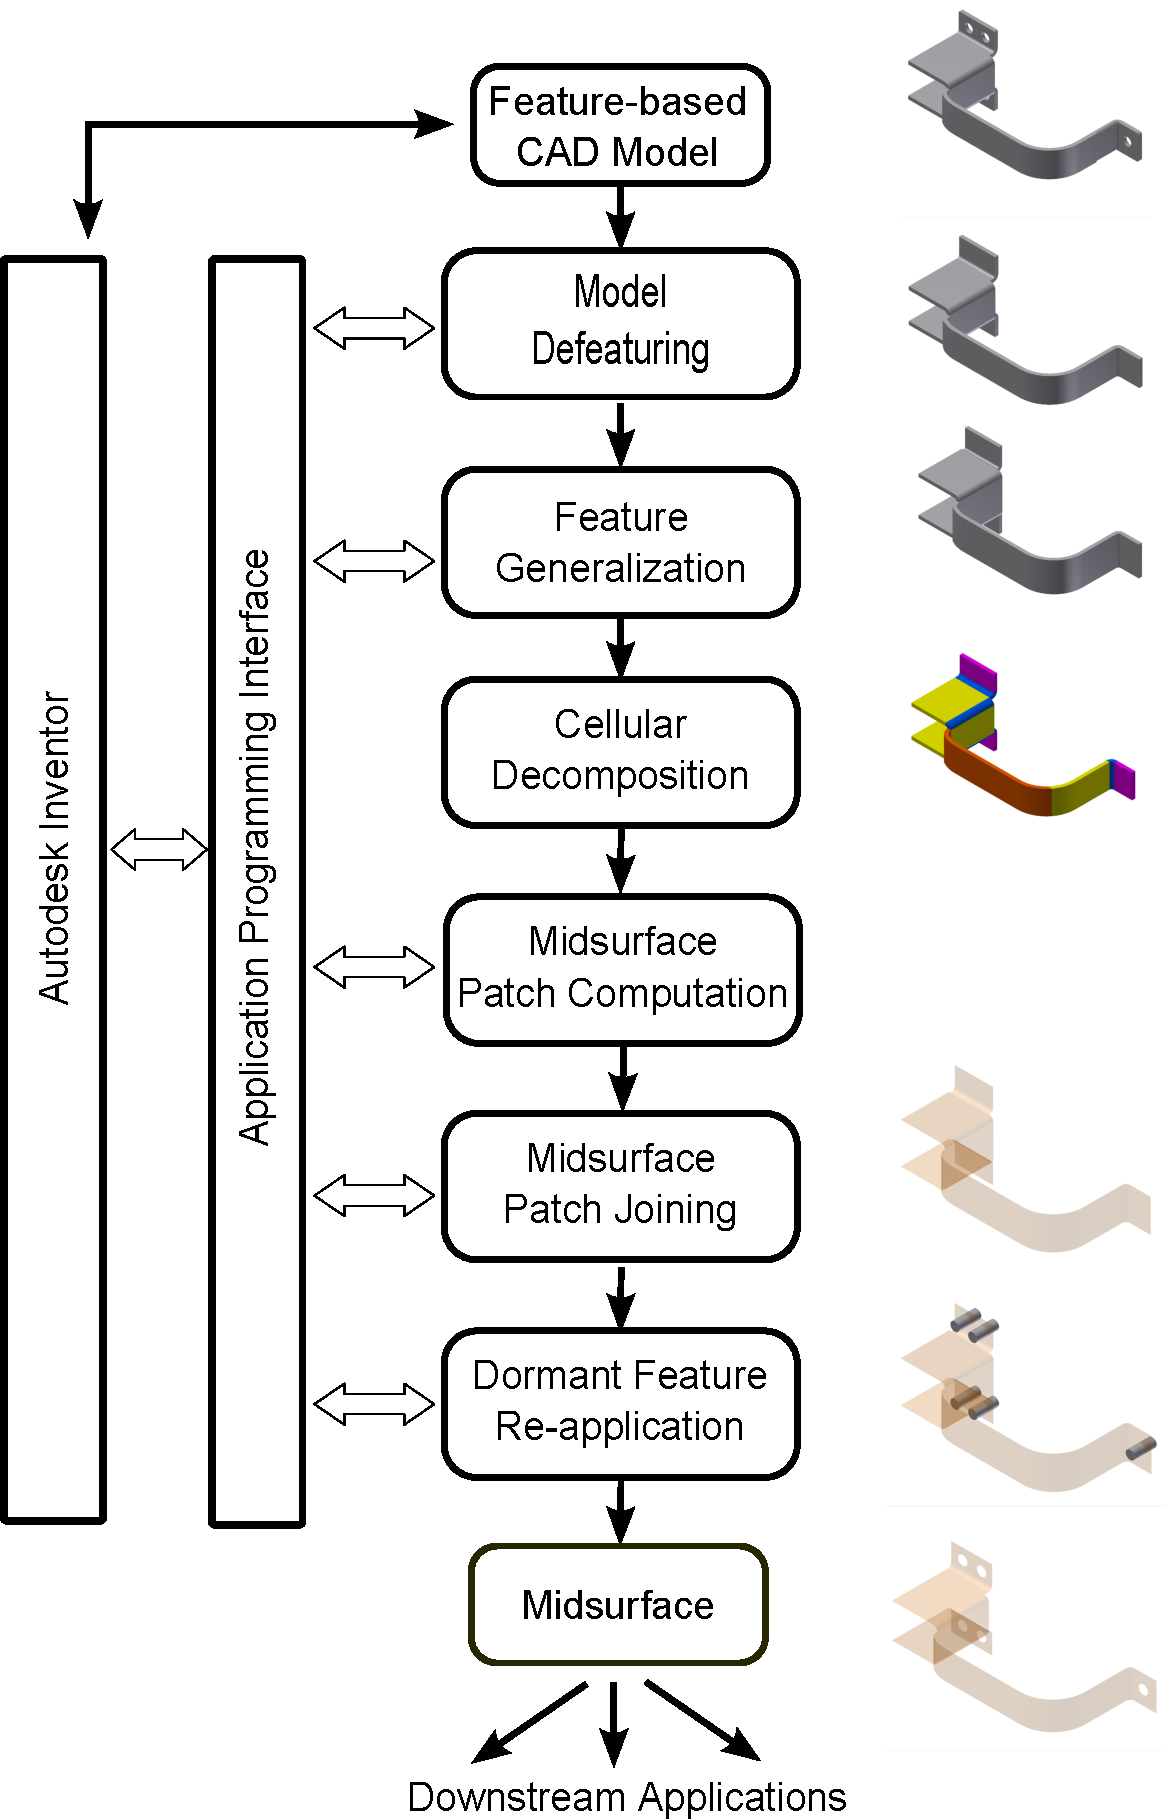
\includegraphics[height=1.05\linewidth]{../Common/images/SystemArchitecture_nolabels_7.pdf}
\vspace{0.5em}

\begin{itemize}[noitemsep,nolistsep]
		\item \textbf{Input}: Feature-based CAD model
		\item \textbf{Defeaturing}: Removes small features
		\item \textbf{Abstraction}: Transforms to generic Sweeps
		\item \textbf{Decomposition}: Forms cellular bodies' graph
		\item \textbf{Midsurface} Interfaces nodes connect midsurface patches created at the non-interface nodes.
\end{itemize}

The output midsurface is far well-connected.

%\vspace{-1.5em}
%	
%
%\begin{figure}[!h]
%\centering 
%\subfloat[Input]{\label{fig_orig}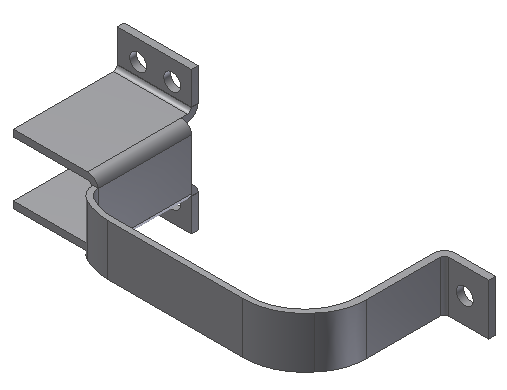
\includegraphics[width=0.3\linewidth,valign=t]{../Common/images/nonCellularBracket}}
%\subfloat[Decompose]{\label{fig_cd}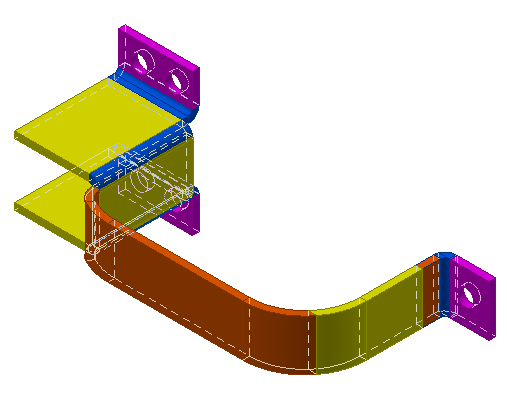
\includegraphics[width=0.3\linewidth,valign=t]{../Common/images/CellularBracket}}
%\subfloat[Midsurface]{\label{fig_mids}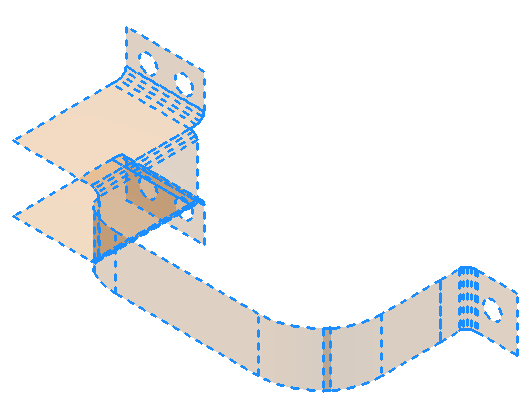
\includegraphics[width=0.3\linewidth,valign=t]{../Common/images/midsCellularBracket}}
%\end{figure}
%
\vspace{-1em}

\section{Papers Published}
\begin{itemize}[noitemsep,nolistsep]
	\item \textbf{Intl Conf, CoEP, 2013}: Feature Midsurface
	\item \textbf{Intl Conf, IITM, 2013}: Defeaturing
	\item \textbf{Intl Conf, IITG, 2014}:  Feature Abstraction
	\item \textbf{Intl Conf, London, 2016}:  Defeaturing
	\item \textbf{Intl Jrnl, Taylor \& Francis, 2015}: Topology
	\item \textbf{Intl Jrnl, T \& Francis, 2015}: Defeature
	\item \textbf{Intl Jrnl, Inderscience, 2017}: Midcurve
	\item \textbf{Intl Jrnl, ASME, 2017}: Midsurface
	\item \textbf{Intl Jrnl, Springer, 2017}: Midsurface
\end{itemize} 

\end{document}